\chapter{Literature Review}

\section{History and Motivation}

Historically, in language technologies and modeling, morphology has been somewhat under-emphasized. This is probably due at least in part to the below-average morphological complexity of English. \parencite{Cotterell2017} English lexemes have relatively few inflected forms, so occurrences of out-of-vocabulary inflected forms are less frequent. And even with grammatical information thrown out via lemmatization, English may still be fairly sensible.

However, in many languages grammatical inflection carries much more semantic burden, and the number of possible inflected forms can be much greater. For instance, a single verb in the Archi language can be inflected in 1,725 ways. \parencite{Cotterell2016} For such highly inflected languages, data sparsity is a significant problem for language models naive to morphology. In languages with a high number of possible forms per lexeme, a much larger number out-of-vocabulary (OOV) are inevitably encountered in test data, requiring reliance on a model's representation of OOV words. Even inflected forms that do occur in training data may not appear often enough for a naive model to understand their semantic content. A model that considers grammatical categories separately is better able to understand the semantic content of inflected words. \parencite{Cotterell2016} It has been empirically shown that comprehending grammatical categories and inflection improves outcomes in language modeling. \parencite{Faruqui2015}

\section{Machine learning of morphology: sub-problems and related problems}

Within the realm of machine understanding of morphology, there are many sub-problems and related problems. The most basic areas of research involve predicting the morphology of words in isolation - transforming a word into a specific morphological form, or the inverse, tagging a form with its morphological categories. Typically, this has been done with words in regular grammatical paradigms, such as number and case marking on nouns, or tense, aspect, mood, and/or argument agreement patterns on verbs. 

\subsection{Core supervised learning problems}

Some of the earliest work in computational morphology involves making specific morphological transformations. That is, given a particular form of a lexeme (often, but not necessarily, a citation form), predicting another form. An example would be learning to pluralize English nouns, e.g., \textit{show} $\rightarrow$ \textit{showed}, \textit{see} $\rightarrow$ \textit{saw}, etc. \parencite{Dreyer2008}

The natural extension of this is aiming to be able to predict any inflected form given a one form and an arbitrary set of morphological categories. Generally speaking, a citation form has been used as input. \parencite{Durrett2013} \parencite{Faruqui2015} \parencite{Cotterell2017} The related "reinflection" problem involves being given any inflected form as input, and transforming it into any other. \parencite{Cotterell2016}

A further extension of the morphology generation problem is the generation of complete inflection tables. The exact nature of this problem depends on the type of training and test data used. If a model is only trained on a sparse, random sampling of forms for each lexeme, then a task may consist of filling out the rest of an inflection table for those lexemes. If a model is trained using entire inflection tables, then test data must consist of new lexemes. Another dimension along which paradigm completion tasks differ is whether only a single citation form is provided as a prompt, or whether any form or even multiple forms may be provided as a prompt for producing a single table. \parencite{Hulden2014} \parencite{Ahlberg2015} \parencite{Cotterell2017} 

Overall, a diverse set of inflection shapes have been worked with. SIGMORPHON 2018 included data from 103 typologically diverse languages, and paradigms using suffixing, prefixing, infixing, reduplication, and non-concatenative morphology. However, all work has been with well-defined, tabular paradigms of fairly moderate size ($\leq 200$ forms). \parencite{Cotterell2018b} Other types of morphology such as derivational morphology and cliticization, which have the potential to greatly expand the number of possible forms and in a less organized fashion, have been less well explored. Highly synthetic languages with more expansive types of word building, including incorporation and productive derivational morphology, are ripe for future work. \parencite{Cotterell2016} 

\subsection{Related problems}

Within only the last two or so years, there has been work on predicting morphology in context. In the 2018 and 2019 SIGMORPHON shared tasks, to which several teams of researchers submitted solutions, a sub-task was dedicated to cloze challenges in which one word in a sentence, given in citation form, was to be inflected based on context. \parencite{Cotterell2018b} \parencite{McCarthy2019} This work is essentially a synthesis of morphology generation and morphosyntactic modeling.

Since 2017, there has been some work done on learning curves for computational morphology. The datasets published for SIGMORPHON 2017 and 2018 include partitions into low ($\sim$100 forms), medium ($\sim$1000 forms), and high ($\sim$10,000 forms) data training sets for the express purpose of assessing the learning curve of different models. The most successful models with high-data training sets are LSTM neural models, generally considered the state of the art model type, yet these often fare worse than baseline string transduction models with low data training sets. \parencite{Cotterell2017} \parencite{Cotterell2018b} Improving performance with small training sets is of interest, as much of the applicability of computational morphology models is to languages which don't already have high-quality technical tools or datasets. 

The most recent new challenge that SIGMORPHON has tried to address is that of transfer learning of morphology, in the shared task earlier this year. Given a state of the art model trained on a language with a high volume of training data, teams were asked to alter it into a model that would perform well on a new language, given a smaller amount of training data for that language. 80\% of the pairs of languages were closely related, while 20\% were distantly or not at all related. Gains of transfer learning models between closely related languages generally performed better than transfer learning models between more distant languages. \parencite{McCarthy2019} 

\section{Non-neural approaches}

\subsection{Vector embedding}

Representing words in relatively low-dimensional vector spaces, with the intention of capturing semantic and syntactic content in a principled way, has found success in a variety of computational linguistics tasks. Regularities in the relative location of semantically related words have been exploited for semantic analysis tasks. \parencite{Bilmes2003} \parencite{Alexandrescu2006}.

Similarly, morphological changes may appear as spatial transformations in vector space, and work has been done on discovering morphological relationships between in-vocabulary words based on their relative spatial locations. This method has the limitation that it cannot extend to words for which a vector representation has not been trained, and so it cannot provide understanding of the many OOV forms encountered in test data of highly inflected languages. \parencite{Mikolov2013} \parencite{Soricut2015} \parencite{DosSantos2014} \parencite{Cotterell2019} 

\begin{figure}[t]
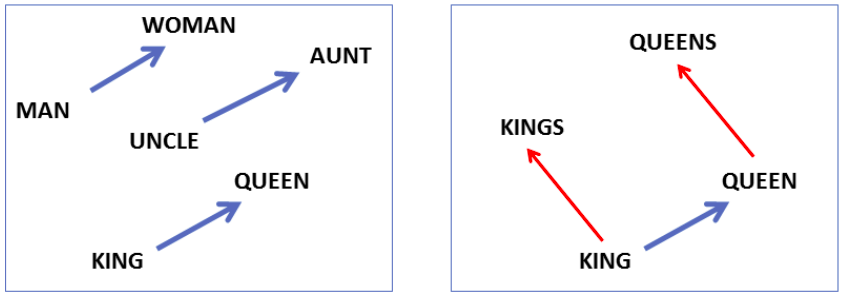
\includegraphics[width=12cm]{images/semantic_transform.png}
\centering
\caption{Regular spatial transformations encode semantic or grammatical content \parencite{Mikolov2013}}
\end{figure}

\subsection{String transduction}

\section{LSTM and other neural approaches}

Since 2016, almost all work on paradigm completion has made use of long short-term memory (LSTM) or related gated recurrent network (GRU) models. \parencite{Faruqui2015} \parencite{Cotterell2016} \parencite{Cotterell2017} \parencite{Cotterell2018b} \parencite{McCarthy2019} In high-data training settings, encoder-decoder LSTMs have proven over the course of annual SIGMORPHON shared tasks to be the state of the art method of computational morphology. However, they have worse performance with sparse training data, an issue which has seen attempts to address.

%% Basic figure template:
%\begin{figure}
%    \centering
%    \includegraphics[width=3in]{figurename.png}
%    \caption{Demo Figure}
%    \label{fig:yourname}
%\end{figure}


%% Basic algorithm template:
%\begin{algorithm}
%\caption{Algorithm Name}
%		\label{alg}
%		\begin{algorithmic}[1]
%			\Procedure{f}{}
%			\State $x$ = initialized variable
%			\For {i = 1 to n}
%	    	\State $x$ = $i$ + 1
%            \EndFor
%		    \State\Return $x$
%			\EndProcedure
%		\end{algorithmic}
%\end{algorithm}


